\subsection{Selected Architectural Styles And Patterns}
In the following section, the selected architectures and design patterns for the implementation phase of the system shall be discussed. Due to nature of the system as a whole and of the services expected to be provided to the users of the system; particularly, the fact that the system provides multiple services which are only connected through the data being produced and consumed by each of them, the system design decisions provided in this section are mostly due to the clear need for decoupling of the various services among each other and their decoupling from the client-side of the system. To be more precise, this system shall adopt the \emph{Microservices Architecture} and the \emph{MVP} design pattern, with the use of \emph{RESTful APIs}. In the hereinafter subsections these design decisions shall be explored.

\subsubsection{Microservices Architecture}
The first of the design decisions to be implemented is the \emph{Microservices} architectural style which subdivides the system into smaller services each of which has limited interaction with other services and provides a unique service to the clients. It is evident that this architectural style perfectly fits the previously described nature of the system. This architectural style not only provides decoupling of the services from the user but also among themselves. Moreover, the architecture at hand is rather scalable with the respect to the number of users since multiple instances of the various microservices may be instantiated to serve the users which is rather simple due to their stateless nature. Below is a figure representing the \emph{Microservices} architectural style, in which the previously discussed aspects of the architecture can be seen.

\begin{figure}[H]
\caption{Microservices Architectural Style (Microsoft Azure 2019)}
\label{fig:MS-arch-style}
\centering
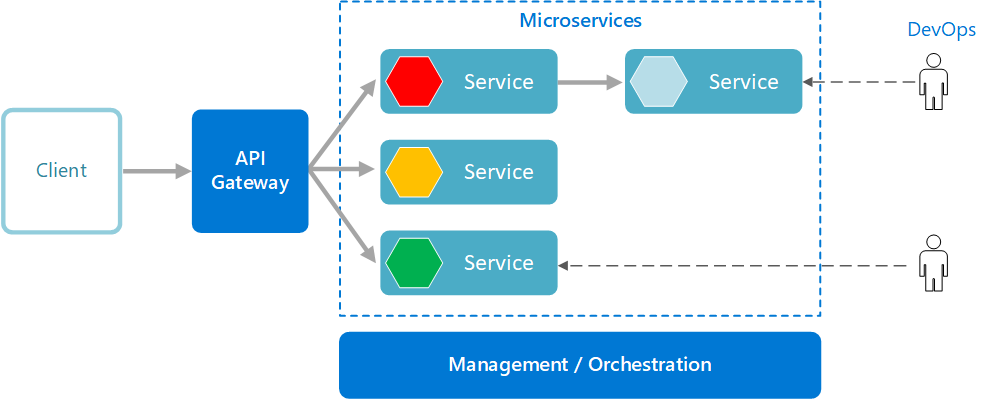
\includegraphics[width=\textwidth, height=0.90\textheight]{microservices-logical.png}
\end{figure}

\subsubsection{Model View Presenter}
In this subsection the design pattern to be used in the system implementation shall be discussed; in particular, the \emph{\textbf{M}odel \textbf{V}iew \textbf{P}resenter (MVP)} design pattern. This design pattern subdivides the system into three general segments; the \emph{Model} representing the business logic and the data, the \emph{View} which interacts directly with user, and the \emph{Presenter} which has a two way interaction with both the view and model; presenting data from the model to the View and manipulating the model based on the user interaction with view. By definition, the \emph{MVP} completely decouples the View and the Presenter and their communication is completely through interfaces; which brings us to the third of the decisions to be discussed in this section later on. The following figure shows the interaction between the system sub-parts as defined by the \emph{MVP} pattern.

\begin{figure}[H]
\caption{MVP Design Pattern}
\label{fig:MVP-desgn-patt}
\centering
\includesvg[width=\textwidth, height=0.8\textheight]{"MVP.svg"}
\end{figure}

\subsubsection{RESTful APIs}
This third and last subsection is concerned with the use of \emph{RESTful APIs} for the interaction between the client and server sides. These APIs can be viewed as the final piece of the puzzle that is the system architecture as a whole. Since the nature of the \emph{RESTful APIs,} falls so perfectly into the system architecture described up to this point. Some of the main properties of these APIs which prove to be rather relevant to this architecture is the fact that they are stateless and flexible in the sense that the data is tied to neither resources nor methods enabling simple scaling with concurrent calls. Therefore, these aspects enable \emph{RESTful APIs} to be a perfect fit for the role of interfacing the View and the Presenter described in the previous subsection. 
